\section{Background}
\label{s:background}

%While concurrency has been a cornerstone of performance benefits in
%the multicore era, it leaves a risk of malfunction, \ie, concurrency
%bug, caused by insufficient thought of concurrent events.
%

Fuzzing is an automated vulnerability discovery technique which has
proven its effectiveness by discovering numerous vulnerabilities in
various softwares such as the Linux kernel.

In this section, we introduce conventional fuzzing approaches to
discover vulnerabilities in the kernel~(\autoref{ss:kernelfuzzing}),
followed by recent improvements in discovering concurrency
bugs~(\autoref{ss:concurrencyfuzzing}).



% \subsection{Concurrency Bug}
% \label{ss:concurrencybugs}
% A concurrency bug is a bug that manifests depending on the timing of
% concurrent events (\eg, memory accesses) that access shared data.
% %
% More specifically, two instructions \textit{conflict} if \textbf{1)}
% they access the same memory location, \textbf{2)} at least one of them
% is a store operation, and \textbf{3)} they are executed concurrently.
% %
% Then, a concurrency bug manifests depending on interleaving order of a
% set of conflicting instructions.

% A concurrency bug is


% \dr{TODO: define conflicting accesses somewhere}

% A concurrency bug can be classified into two categories according to
% how it adversely affects a program.

% \begin{figure}
%   \centering
%   \subfloat[Data race.\label{subfig:datarace}] {
%     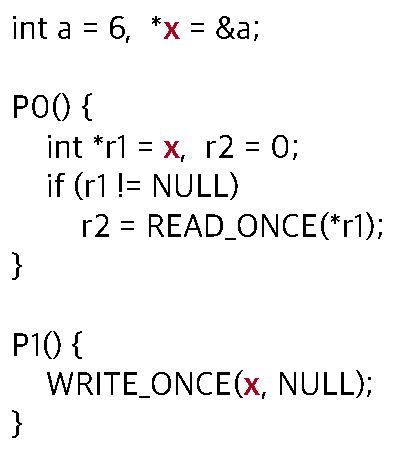
\includegraphics[width=0.45\linewidth]{fig/datarace.pdf}
%   }
%   \hfill
%   \subfloat[Race condition.\label{subfig:racecondition}] {
%     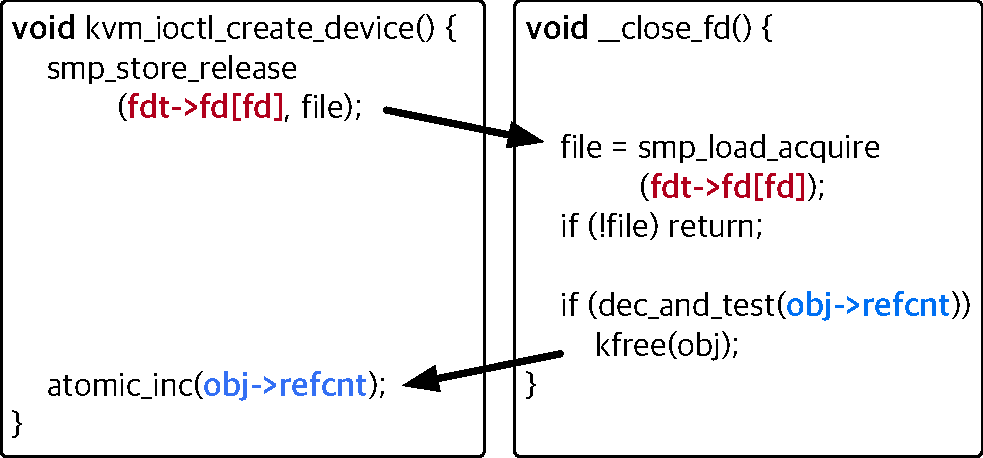
\includegraphics[width=0.45\linewidth]{fig/racecondition.pdf}
%   }
%   \caption{Two types of concurrency bugs.}
%   \label{fig:concurrencybugs}
% \end{figure}


% \PP{Data race.}
% %
% Although the concept of data race is well known, its formal definition
% depends on a programming language~\cite{C-standard-n2310,
%   java-standard} or a program in development~\cite{lkmm}. In this
% paper, we employ the definition from Linux Kernel Memory Model
% (LKMM)~\cite{lkmm}. According to LKMM, a data race occurs when there
% are two memory accesses such that 1) they access the same location, 2)
% at least one of them is a store, 3) at least one of them is not
% annotated with special operations such as \texttt{WRITE_ONCE()}, or
% \texttt{smp_load_acquire()}, 4) they occur on different CPUs (or in
% different threads on the same CPU), and 5) they execute concurrently.
% %
% Informally, a data race indicates un-annotated concurrent accesses to
% a shared memory location.

% Data races are problematic because they may confuse a compiler.  LKMM
% allows a compiler to assume that there will be no data race during the
% runtime. Based on the assumption, a compiler has its rights to
% arbitrarily transform plain accesses (\ie, accesses not annotated with
% above operations), making the results unpredictable if there is a data
% race during the runtime.
% %
% Therefore, LKMM defines the outcome of the program as undefined
% behavior if a data race occurs.
% %
% Also, to prevent such undefined behaviors, LKMM requires developers to
% annotate accesses if they possibly run
% concurrently~\cite{data-race-fix1, data-race-fix2, data-race-fix3}.
% % %
% % On the other hand, data races may or may not cause a real-world issue
% % such as memory corruption. Many data races fixes~\cite{data-race-fix1,
% %   data-race-fix2, data-race-fix3} annotate memory accessing
% % instructions with above operations, which actually does not affect the
% % compiled binary.


% \PP{Race condition.}
% %
% Race condition is another type of concurrency bug. While a race
% condition broadly indicates that an outcome differs depending on the
% timing of concurrent events, we restrict the definition to indicate
% the correctness of the outcome differs according to the timing of
% concurrent events.
% %
% Specifically, if developers do not take consider of all possible
% interleavings, a program may execute an erroneous interleaving which
% leads the program into an unintended state.
% %
% Immediately or after a certain amount of time, the unintended state
% causes erroneous behaviors of the program such as memory corruption,
% deadlock, and assertion violation.

% % \dr{TODO: what more?}
% % In order to fix the errorneous interelaving, developers often utilize
% % synchronization primitives such as a lock, or switch the order of
% % instructions in a program~\cite{learningfrommistakes}.


% % https://stackoverflow.com/questions/11276259/are-data-races-and-race-condition-actually-the-same-thing-in-context-of-conc
% %
% \PP{Differences between data race and race condition}
% %
% \dr{TODO: rewrite to enphasize that finding race condition is
%   important and combine this into the race condition paragraph}
% %
% Although both race condition and data race are a bug caused by
% concurrenct events, there are a few differences.
% %
% First, a data race is regards to a single pair of conflicting accesses
% while a race condition is about an interleaving.
% %
% Therefore, methods to detect them are also different.  While data race
% detectors~\cite{tsan, krace, prorace, crsampler, txrace} monitor
% whether two conflicting plain accesses are executed concurrently, race
% conditions can be observed only through an erroneous behavior caused
% by a specific interleaving.
% %
% Second, whereas a data race occurs if such conflicting accesses exists
% no matter it causes an erroneous behavior or not, a race condition is
% told by an abnormal outcome of a program.
% %
% % In the security perspective, a data race requires further
% % investigation to determine whether it is harmful or
% % not~\cite{portend, replayanalysis}, the effect of a race condition
% % is exmained by erroneous behaviors such as general protection fault,
% % assertion violations, sanitizers~\cite{asan, kasan} and
% % lockdep~\cite{lockdep} reports.
% %
% % \begin{figure}
% %   \centering
% %   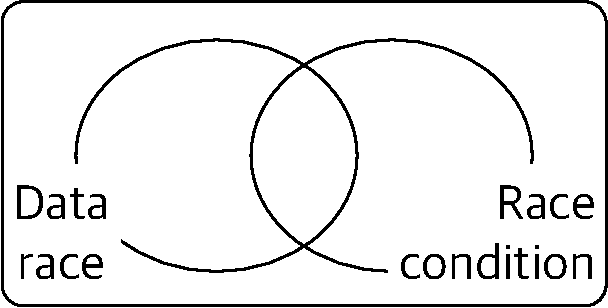
\includegraphics[width=0.45\linewidth]{fig/venndiagram.pdf}
% %   \caption{Relation between data race and race condition. This paper
% %     focuses on the striped region. \dr{I don't think we need this.}}
% %   \label{fig:venndiagram}
% % \end{figure}
% %
% Lastly, they are not a subset or a superset of one another. Although
% there are race conditions that occur with data races, neither one is
% the sufficient nor necessary condition for the other. Therefore, we
% would argue that finding data races and finding race condditions are
% complementary with each other.


% \PP{Scope of this paper}
% %
% This paper focuses on finding race conditions instead of data races.

% \dr{TODO: why? want to say finding race condition is more important,
%   and existing approaches to find data races are limited}

% \dr{TODO: need to say the importance of observing erroneous outcomes}

\subsection{(Conventional) Kernel Fuzzing}
\label{ss:kernelfuzzing}

Throughout decades, a number of fuzzing approaches~\cite{imf,
  syzkaller, moonshine, hfl, healer, janus, hydra, trinity} have been
proposed to discover vulnerabilities in the kernel.
%
These approaches, specifically coverage-guided fuzzing approaches,
execute a massive number of inputs (\ie, sequences of system calls)
while a code coverage metric (\eg, branch coverage) tracks the
execution path that each input explores by using.
%
In addition, during the execution of inputs, a fuzzer detects
vulnerabilities with a help of various sanitizers~\cite{meds, kasan,
  asan, ubsan, lockdep}.


While conventional fuzzing techniques show the practicality even in
large system softwares, they mostly focus on the \textit{sequential
  aspect} of the execution (\ie, the execution path of a single
thread), while the concurrency aspect (\ie, thread interleaving) is
left uncontrolled.
%
% In other words, they are designed to effectively explore source codes
% residing deep inside the kernel without considering how threads are
% interleaved during the execution.
%
As a consequence, conventional fuzzing approaches are limited in
discovering concurrency bugs such as race conditions, data races, and
deadlocks~\cite{covcon, terragni2018effectiveness}.


% What do they do: explore more code path

% How: inputs (= system call sequence)


\subsection{Concurrency Fuzzing}
\label{ss:concurrencyfuzzing}


% During fuzzing, a fuzzer determines that interleavings of given
% concurrent jobs are tested enough if a concurrency coverage is
% saturated while a customized scheduler is introduced to tailor the
% non-deterministic behavior.

% discovering kernel concurrency bugs is still a daunting task.

% %
% It is mainly due to two challenges such that 1) concurrency bugs are
% inherently caused non-deterministically, and 2) the number of
% possible interleavings grows exponentially to the number of memory
% access operations.

Recently, several approaches, classified as concurrency
fuzzing~\cite{razzer, krace, snowboard, muzz, conzzer}, have been
proposed to take consider of the \textit{concurrency aspect} of kernel
execution into the fuzzing process.
%
Concurrency fuzzers generally repeat the execution of a multi-thread
input (\eg, a multi-threaded system call sequence) while 1) capturing
unique behaviors of thread interleavings with a \textit{interleaivng
  coverage metric}, and 2) exploring thread interleavings based on
a \textit{thread interleaving search strategy}.


% \PP{Coverage-guided fuzzing}
% %
% Throughout decades, a fuzzing has shown its ability to find bugs in
% various software layers including the userprogram space~\cite{qsym,
%   driller, crfuzz, r2z2, cafl, fuzzorigin} and the kernel
% space~\cite{fuzzusb, syzkaller, hfl, cabfuzz, razzer, krace, janus,
%   hydra, healer}.
% %
% A primary task of fuzzing is to synthesize and mutate various inputs
% of a target program.
% %
% When running the inputs, a fuzzer monitors a program's behavior, and
% observes malfunctions with a help of various developer
% tools~\cite{asan, kasan, meds}.

% A coverage-guided fuzzer adopts a coverage metric to abstract
% program's interesting behaviors.
% %
% During fuzzing, a fuzzer accumulates all experienced coverage as the
% abstraction of tested behaviors of a program.
% %
% When a new input is given, a fuzzer compares coverage of the input
% with the accumulated coverage to determine whether the input exposes a
% new interesting behavior. If it does, a fuzzer keeps and mutates the
% input to generate another input that potentially exhibits unknown
% coverage.

% \dr{TODO: Do we need to tell about coverage-directed fuzzers?}


\PP{Interleaving coverage metric.}
%
As Krace~\cite{krace} reveals, code coverage metrics (\eg, branch
coverage) are not enough to capture unique behaviors of thread
interleavings. This is because code coverage metrics only track
behaviors in a single thread without paying attention to thread
interleavings (\eg, branch coverage tracks whether a branch is taken
or not in a single thread).


To capture unique behaviors of thread interleavings, a few concurrency
fuzzing approaches~\cite{conzzer, krace} come up with interleaving
coverage metrics.
%
Especially, Krace~\cite{krace} proposes alias coverage as an
interleaving coverage metric, where alias coverage tracks an
instruction pair ($I_S$, $I_L$), if a read instruction $I_L$ reads a
value written by a write instruction $I_S$, and they are executed by
different threads.
%
Whereas, Conzzer~\cite{conzzer} proposes another interleaving coverage
metric called concurrent call pair, where each concurrent call pair
represents a pair of two concurrently-executed functions augmented
with calling contexts.

Concurrency fuzzing approaches aggregate interleaving coverage across
iterations while repeatedly executing a given multi-thread input until
the multi-thread input no longer provides new interleaving coverage.
%
Taking Krace as an example, alias coverage constructs a set of
instruction pairs collected through iterations. When further
iterations do not generate a new instruction pair, Krace
de-prioritizes the multi-thread input to explore thread interleavings
of other multi-thread inputs.



% inter-thread data flow
% between a pair of instructions.
% %
% In other words, alias coverage tracks a directed pair of instructions
% \texttt{$I_S \rightarrow I_L$}, if a load instruction \texttt{$I_L$}
% reads a value written by a store instruction \texttt{$I_S$} and they
% are executed in different threads.
% %
% If Krace no longer finds such instruction pair in a given multi-thread
% input, it concludes that the multi-thread input has been explored
% enough, and de-prioritize the multi-thread input.



% Although Razzer~\cite{razzer} and Snowboard~\cite{snowboard} also
% concentrate on discovering concurrency bugs in the kernel, they do not
% make use of a interleaving coverage metric.
% %
% Therefore they are limited in determining that a given multi-thread
% input needs to be further explored.

% Instead, they concentrate on less frequent inter-thread
% data flow based on an idea that those inter-thread data flow is less
% likely tested and more likely causes an abnormal behavior.


% \dr{TODO: MUZZ, and conzzer?}


\PP{Thread interleaving search strategy}
%
Unlike conventional fuzzing approaches, concurrency fuzzing considers
thread scheduling is another input domain that a fuzzer needs to
explore.
%

To determine which thread interleaving to run for each iteration, a
fuzzer adopts a thread interleaving search strategy (shortly, an
interleaving search strategy).
%
For instance, Razzer~\cite{razzer} and Snowboard~\cite{snowboard}
picks a single pair of instructions (\eg, \texttt{X} and \texttt{Y})
that access the same memory object and test their execution order,
\eg, executing \texttt{X} before \texttt{Y}.
%
Whereas, Krace~\cite{krace} randomly determins a thread interleaving
to run for each execution.
%
\dr{Conzzer and MUZZ?}



After determining a thread interleaivng to run,w concurrency fuzzing
overrides the kernel scheduler, and controls thread scheduling as
desired.
%
To this end, a thread scheduling control mechanism is used to control
thread scheduling as a fuzzer wants. Depending on a concurrency
fuzzer, various mechanisms are used;
%
Razzer~\cite{razzer} and Snowboard~\cite{snowboard} suspend and resume
virtual CPUs on which target threads are running, Krace~\cite{krace}
and Conzzer~\cite{conzzer} inject delays before memory accesses
through instrumentation and the breakpoint feature respectively.
%
While these methods are designed differently, all of them allow a
fuzzer to control thread scheduling.



% \dr{TODO: rewrite}

% Depending on how it schedules instructions, it is largely categorized
% into randomized scheduler and scheduling hint-directed scheduler
% (shortly, hint-directed scheduler).

% A randomized scheduler~\cite{ski, pctalgorithm, krace, sparsernr} is
% designed to randomly schedule intstructions in a disciplined
% manner.
% %
% It tries to keep only one thread to execute while the thread
% runs until a certain number of instructions are executed or a certain
% amount of time has elapsed.
% %
% A fuzzer and the scheduler share a small number of parameters used for
% the scheduler to pseudo-randomly determine the number of instructions
% or the amount of time to execute.
% %
% In this way, interleavings are diversified across fuzzing runs while a
% fuzzer can tailor the non-determinism caused by scheduling.

% On the other side, a hint-directed scheduler~\cite{razzer, snowboard}
% enfoces a specific requirement of interleaving called a scheduling
% hint.
% %
% A scheduling hint is generally in the form of an interleaving pattern
% that possibly causes a concurrency bug. For example, a scheduling hint
% may consists of execution order indicating a single-variable order
% violation; \textit{``thread A executes a store operation writing into
%   $X$ before thread B executes a load operation reading from $X$''}.
% %
% During fuzzing, a fuzzer keeps generating different scheduling hints,
% and enforces an interleaving that contains a scheduling hint to
% observe the interleaving causes an erroneous behavior.


%%% Local Variables:
%%% mode: latex
%%% TeX-master: "p"
%%% End:
